\documentclass[12pt]{article}

%%%%%%%%%%%%%%%%%%%%%%%%%%%%%%%%%%%%%%%%%%%%%%%%%%%%%%%%%%%%%%%%%%%%%%%%%%%%%%%%
%                           Package preset for homework
%%%%%%%%%%%%%%%%%%%%%%%%%%%%%%%%%%%%%%%%%%%%%%%%%%%%%%%%%%%%%%%%%%%%%%%%%%%%%%%%
% Miscellaneous
\usepackage[margin=1in]{geometry}
\usepackage[utf8]{inputenc}
\usepackage{indentfirst}
\usepackage{blindtext}
\usepackage{graphicx}
\usepackage{xr-hyper}
\usepackage{hyperref}
\usepackage{enumitem}
\usepackage{color}
\usepackage{float}
% Math
\usepackage{latexsym}
\usepackage{amsfonts}
\usepackage{amssymb}
\usepackage{amsmath}
\usepackage{commath}
\usepackage{amsthm}
\usepackage{bbold}
\usepackage{bm}
% Physics
\usepackage{physics}
\usepackage{siunitx}
% Code typesetting
\usepackage{listings}
% Citation
\usepackage[authoryear]{natbib}
\usepackage{appendix}
\usepackage[capitalize]{cleveref}
% Title & name
\title{Homework}
\author{Tien Vo}
\date{\today}


%%%%%%%%%%%%%%%%%%%%%%%%%%%%%%%%%%%%%%%%%%%%%%%%%%%%%%%%%%%%%%%%%%%%%%%%%%%%%%%%
%                   User-defined commands and environments
%%%%%%%%%%%%%%%%%%%%%%%%%%%%%%%%%%%%%%%%%%%%%%%%%%%%%%%%%%%%%%%%%%%%%%%%%%%%%%%%
%%% Misc
\sisetup{load-configurations=abbreviations}
\newcommand{\due}[1]{\date{Due: #1}}
\newcommand{\hint}{\textit{Hint}}
\let\oldt\t
\renewcommand{\t}[1]{\text{#1}}

%%% Bold sets & abbrv
\newcommand{\N}{\mathbb{N}}
\newcommand{\Z}{\mathbb{Z}}
\newcommand{\R}{\mathbb{R}}
\newcommand{\Q}{\mathbb{Q}}
\let\oldP\P
\renewcommand{\P}{\mathbb{P}}
\newcommand{\LL}{\mathcal{L}}
\newcommand{\FF}{\mathcal{F}}
\newcommand{\HH}{\mathcal{H}}
\newcommand{\NN}{\mathcal{N}}
\newcommand{\ZZ}{\mathcal{Z}}
\newcommand{\RN}[1]{\textup{\uppercase\expandafter{\romannumeral#1}}}
\newcommand{\ua}{\uparrow}
\newcommand{\da}{\downarrow}

%%% Unit vectors
\newcommand{\xhat}{\vb{\hat{x}}}
\newcommand{\yhat}{\vb{\hat{y}}}
\newcommand{\zhat}{\vb{\hat{z}}}
\newcommand{\nhat}{\vb{\hat{n}}}
\newcommand{\rhat}{\vb{\hat{r}}}
\newcommand{\phihat}{\bm{\hat{\phi}}}
\newcommand{\thetahat}{\bm{\hat{\theta}}}

%%% Other math stuff
\providecommand{\units}[1]{\,\ensuremath{\mathrm{#1}}\xspace}
% Set new style for problem
\newtheoremstyle{problemstyle}  % <name>
        {10pt}                   % <space above>
        {10pt}                   % <space below>
        {\normalfont}           % <body font>
        {}                      % <indent amount}
        {\bfseries\itshape}     % <theorem head font>
        {\normalfont\bfseries:} % <punctuation after theorem head>
        {.5em}                  % <space after theorem head>
        {}                      % <theorem head spec (can be left empty, 
                                % meaning `normal')>

% Set problem environment
\theoremstyle{problemstyle}
\newtheorem{problemenv}{Problem}[section]
\newenvironment{problem}[1]{%
  \renewcommand\theproblemenv{#1}%
  \problemenv
}{\endproblemenv}
% Set lemma environment
\newenvironment{lemma}[2][Lemma]{\begin{trivlist}
\item[\hskip \labelsep {\bfseries #1}\hskip \labelsep {\bfseries #2.}]}{\end{trivlist}}
% Set solution environment
\newenvironment{solution}{
    \begin{proof}[Solution]$ $\par\nobreak\ignorespaces
}{\end{proof}}
\numberwithin{equation}{problemenv}

%%% Page format
\setlength{\parindent}{0.5cm}
\setlength{\oddsidemargin}{0in}
\setlength{\textwidth}{6.5in}
\setlength{\textheight}{8.8in}
\setlength{\topmargin}{0in}
\setlength{\headheight}{18pt}

%%% Code environments
\definecolor{dkgreen}{rgb}{0,0.6,0}
\definecolor{gray}{rgb}{0.5,0.5,0.5}
\definecolor{mauve}{rgb}{0.58,0,0.82}
\lstset{frame=tb,
  language=Python,
  aboveskip=3mm,
  belowskip=3mm,
  showstringspaces=false,
  columns=flexible,
  basicstyle={\small\ttfamily},
  numbers=none,
  numberstyle=\tiny\color{gray},
  keywordstyle=\color{blue},
  commentstyle=\color{dkgreen},
  stringstyle=\color{mauve},
  breaklines=true,
  breakatwhitespace=true,
  tabsize=4
}
\lstset{
  language=Mathematica,
  numbers=left,
  numberstyle=\tiny\color{gray},
  numbersep=5pt,
  breaklines=true,
  captionpos={t},
  frame={lines},
  rulecolor=\color{black},
  framerule=0.5pt,
  columns=flexible,
  tabsize=2
}


\title{Homework 6: Phys 7310 (Fall 2021)}

\begin{document}
\maketitle

%%%%%%%%%%%%%%%%%%%%%%%%%%%%%%%%%%%%%%%%%%%%%%%%%%%%%%%%%%%%%%%%%%%%%%%%%%%%%%%%
\begin{problem}{6.1}[The potential inside a cylinder]
(a) A hollow right circular cylinder of radius $b$ has its axis coincident with 
the $z$ axis and its ends at $z=0$ and $z=L$. The potential on the end faces is
zero, while the potential on the cylindrical surface is given as $V(\phi,z)$.
Using the appropriate separation of variables in cylindrical coordinates, find a
series solution for the potential anywhere inside the cylinder.

(b) For the cylinder in the previous part, the cylindrical surface is made of
two equal half-cylinders, one at potential $V$ and the other at potential $-V$,
so that
\begin{equation}\label{p1:V}
    V(\phi,z)=\begin{cases}
        V, & \phi\in(-\pi/2,\pi/2)\\
        -V, & \phi\in(\pi,2,3\pi/2)
    \end{cases}
\end{equation}
Find the potential inside the cylinder.
\begin{solution}
(a) By separation of variables, we write
$\Phi(\rho,\phi,z)=R(\rho)Q(\phi)Z(z)$ and plug back into Laplace equation
\begin{equation}
    \frac{R''}{R}+\frac1{\rho}\frac{R'}{R}+\frac1{\rho^2}\frac{Q''}{Q}+\frac{Z''}{Z}=0
\end{equation}
Because $Z$ has to vanish at finite $z$, we can let $Z''(z)=-k^2Z(z)$ for some
constant $k$, the general solution to which is
\begin{equation}
    Z(z)=a\cos(kz)+b\sin(kz) 
\end{equation}
The boundary conditions require that $Z(0)=a=0$ and $Z(L)=b\sin(kL)=0$. The
latter makes $k$ discrete $k_n=n\pi /L$ for some $n\in\qty{1,2,3,\ldots}$. Now, 
our differential equation becomes
\begin{equation}
\rho^2\frac{R''}{R}+\rho\frac{R'}{R}-k^2\rho^2+\frac{Q''}{Q}=0
\end{equation}
Letting $Q''(\phi)=-\nu^2Q(\phi)$, the solution for $Q$ is
$A\cos(m\phi)+B\sin(m\phi)$. Then the differential equation in $\rho$ is
\begin{equation}
    R''(\rho)+\frac1\rho R'(\rho)-\qty(k^2+\frac{\nu^2}{\rho^2})R(\rho)=0
\end{equation}
Let $x=k\rho$, the solution for $R$ is then
\begin{equation}
    R(\rho)=CI_\nu(k\rho)+DK_\nu(k\rho)
\end{equation}
for $\nu\in\N$. Since $K_\nu\to\infty$ for $\rho\to 0$, $D$ has to be zero 
because the potential is finite in the cylinder. Combining the previous 
results, the general solution to the potential is
\begin{equation}\label{p1a:Phi}
    \Phi(\rho,\phi,z)=\sum_{m=0}^\infty\sum_{n=1}^\infty
    I_m(k_n\rho)[A_{nm}\cos(m\phi)+B_{nm}\sin(m\phi)]\sin\qty(\frac{n\pi z}{L})
\end{equation}
Now, applying the last boundary condition, we can write
$\Phi(b,\phi,z)=V(\phi,z)$ and
\begin{equation}
    V(\phi,z)=\sum_{m'=0}^\infty\sum_{n'=1}^\infty
    I_{m'}(k_{n'}b)\qty[A_{n'm'}\cos(m'\phi)+B_{n'm'}\sin(m'\phi)]\sin\qty(\frac{n'\pi z}{L})
\end{equation}
Multiplying both sides with $2 /\pi L\cos(m\phi)\sin(n\pi z /L)$ and
integrating, we can write from the orthogonality condition
\begin{equation}
    \frac2{\pi L}\int_0^L\int_0^{2\pi}V(\phi,z)\cos(m\phi)\sin\qty(\frac{n\pi
    z}{L})d\phi dz=\sum_{m'=0}^\infty\sum_{n'=1}^\infty I_{m'}(k_{n'}b)
    A_{n'm'}\delta_{mm'}\delta_{nn'}=I_m(k_nb)A_{nm}
\end{equation}
Thus,
\begin{equation}
    A_{nm}=\frac2{\pi L}\frac1{I_m(n\pi
    b/L)}\int_0^L\int_0^{2\pi}V(\phi,z)\cos(m\phi)\sin\qty(\frac{n\pi
z}{L})d\phi dz 
\end{equation}
Similarly,
\begin{equation}
    B_{nm}=\frac2{\pi L}\frac1{I_m(n\pi
    b/L)}\int_0^L\int_0^{2\pi}V(\phi,z)\sin(m\phi)\sin\qty(\frac{n\pi
z}{L})d\phi dz 
\end{equation}
Then we can rewrite the solution \eqref{p1a:Phi} as
\begin{equation}
    \Phi(\rho,\phi,z)
    =\frac2{\pi L}\sum_{m=0}^\infty\sum_{n=1}^\infty
    \frac{I_m(n\pi \rho/L)}{I_m(n\pi
    b/L)}\qty[a_{nm}\cos(m\phi)+b_{nm}\sin(m\phi)]\sin\qty(\frac{n\pi z}{L})
\end{equation}
where
\begin{subequations}\label{p1a:coeff}
    \begin{align}
        a_{nm}
        &=\int_0^L\int_0^{2\pi}V(\phi',z')\cos(m\phi')\sin\qty(\frac{n\pi
        z'}{L})d\phi'dz'\\ 
        b_{nm}
        &=\int_0^L\int_0^{2\pi}V(\phi',z')\sin(m\phi')\sin\qty(\frac{n\pi
        z'}{L})d\phi'dz'
    \end{align} 
\end{subequations}

(b) With the potential as in \eqref{p1:V}, the coefficients \eqref{p1a:coeff} 
for $m=0$ become
\begin{subequations} 
    \begin{align}
        a_{n0}&=
            V\int_0^L\sin\qty(\frac{n\pi z'}{L})dz'
            \qty[\int_{-\pi/2}^{\pi/2}d\phi'-\int_{\pi/2}^{3\pi/2}d\phi']=0\notag\\
        b_{n0}&=0
    \end{align}
\end{subequations}
For $m\neq 0$,
\begin{subequations}
    \begin{align}
        a_{nm}
        &=\frac{4VL}{mn\pi}\qty[1-(-1)^n]\sin^3\qty(\frac{m\pi}{2})\label{p1b:anm}\\
        b_{nm}
        &=-\frac{2VL}{mn\pi}\qty[1-(-1)^n]\sin\qty(\frac{m\pi}{2})\sin\qty(m\pi)
        =0
    \end{align} 
\end{subequations}
From \eqref{p1b:anm}, the only non-trivial terms have $n,m\in 2\N+1$ (odd). Then
we can write the solution as
\begin{equation}
    \Phi(\rho,\phi,z)
    =\frac{8V}{\pi^2}\sum_{n,m\in
    2\N+1}\frac{\qty[1-(-1)^n]}{mn}\frac{I_m(n\pi\rho/L)}{I_m(n\pi b/L)}
        \sin^3\qty(\frac{m\pi}{2})\cos(m\phi)\sin\qty(\frac{n\pi z}{L})
\end{equation}
\end{solution}
\end{problem}
%%%%%%%%%%%%%%%%%%%%%%%%%%%%%%%%%%%%%%%%%%%%%%%%%%%%%%%%%%%%%%%%%%%%%%%%%%%%%%%%
%%%%%%%%%%%%%%%%%%%%%%%%%%%%%%%%%%%%%%%%%%%%%%%%%%%%%%%%%%%%%%%%%%%%%%%%%%%%%%%%
\begin{problem}{6.2}[Multiple moments]
Calculate the multipole moment $q_{lm}$ of the charge distributions shown as
parts a and b. Try to obtain results for the nonvanishing moments valid for all
$l$, but in each case find the first \textit{two} sets of nonvanishing moments
at the very least.
\begin{center}
    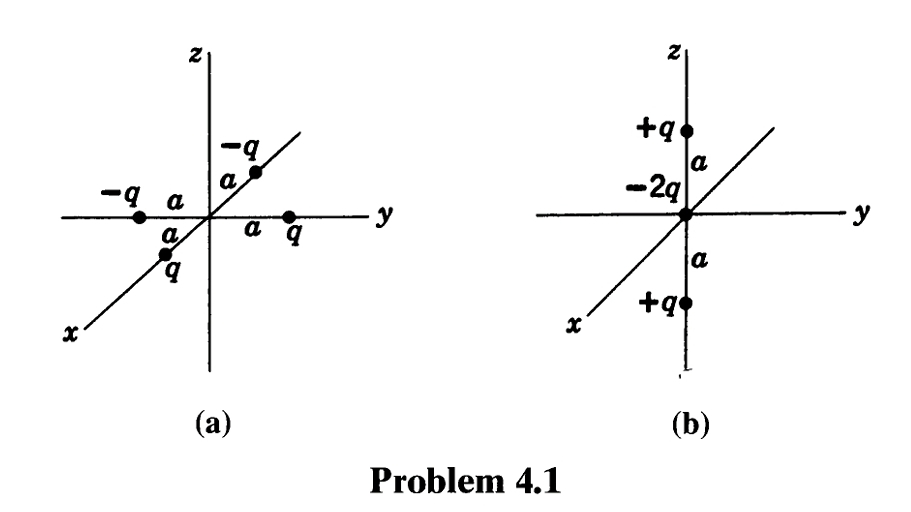
\includegraphics[width=0.7\textwidth]{hw6_p2.jpg} 
\end{center}

(c) For the charge distribution of the second set b write down the multipole
expansion for the potential. Keeping only the lowest-order term in the
expansion, plot the potential in the $xy$ plane as a function of distance from
the origin for distances greater than $a$.

(d) Calculate directly from Coulomb's law the exact potential for $b$ in the
$xy$ plane. Plot it as a function of distance and compare with the result found
in part c.

Divide out the asymptotic form in parts c and d to see the behavior at large
distances more clearly.
\begin{solution}
(a) The charge density in spherical coordinates can be written as
\begin{equation}
    \rho(\vb{x}')=q\frac{\delta(r'-a)}{r'^2}\delta(\cos\theta')
    \qty[\delta(\phi')+\delta\qty(\phi'-\frac\pi2)-\delta(\phi'-\pi)-\delta\qty(\phi'+\frac\pi2)]
\end{equation}
Then the multipole moment is, by definition
\begin{align}
    q_{lm}
    &=q\sqrt{\frac{2l+1}{4\pi}\frac{(l-m)!}{(l+m)!}}
    \int_0^\infty r'^l\delta(r'-a)dr'
    \int_{-1}^1P_l^m(\cos\theta')\delta(\cos\theta')d(\cos\theta')\notag\\
    &\qquad\times\int_0^{2\pi}e^{-im\phi'}\qty[\delta(\phi')+\delta\qty(\phi'-\frac\pi2)-\delta(\phi'-\pi)-\delta\qty(\phi'+\frac\pi2)]d\phi'\notag\\
    &=q\sqrt{\frac{2l+1}{4\pi}\frac{(l-m)!}{(l+m)!}}
        a^lP_l^m(0)\qty[1+e^{-im\pi/2}-e^{-im\pi}-e^{im\pi/2}]\notag\\
    &=qa^l\sqrt{\frac{2l+1}{4\pi}\frac{(l-m)!}{(l+m)!}}
    (-1)^m\qty[1-(-1)^m-2i\sin\qty(\frac{m\pi}{2})]\eval{\frac{d^m}{dx^m}P_l(x)}_{x=0}
\end{align}
Note from the square bracket that $m$ has to be odd so that it does not vanish.
Then $d^mP_l /dx^m$ is an odd polynomial if $l$ is even. However, odd
functions vanish at $x=0$. So $l$ has to also be odd if $m$ is odd. Thus,
$l,m\in 2\N+1$. We can then write
\begin{equation}
    q_{lm}=2qa^l\sqrt{\frac{2l+1}{4\pi}\frac{(l-m)!}{(l+m)!}}P_l^m(0)\qty[1-i\sin\qty(\frac{m\pi}{2})] 
\end{equation}
Up to $l=3$, the only non-trivial terms (with $m\geq 0$) are
\begin{equation}
    q_{11}=qa\sqrt{\frac{3}{2\pi}}(-1+i),
    \qquad q_{31}=\frac{qa^3}{4}\sqrt{\frac{21}{\pi}}(1-i),
    \qquad\text{and}\qquad
    q_{33}=-\frac{qa^3}{4}\sqrt{\frac{35}{\pi}}(1+i)
\end{equation}

(b) The charge density in spherical coordinates is
\begin{equation}
    \rho(\vb{x}')=\frac{q}{2\pi}\frac1{r'^2}\qty{\delta\qty(r'-a)\qty[\delta(\cos\theta'-1)+\delta(\cos\theta'+1)]-\delta(r')} 
\end{equation}
Then by definition, the multipole moment is
\begin{align}\label{p2b:q}
    q_{lm}
    &=\frac{q}{2\pi}\sqrt{\frac{2l+1}{4\pi}\frac{(l-m)!}{(l+m)!}}
    \int_0^{2\pi}e^{-im\phi'}d\phi'\Bigg\{\notag\\
    &\qquad\int_0^\infty dr'r'^l\delta(r'-a)
        \int_{-1}^1d(\cos\theta')P_l^m(\cos\theta')\qty[\delta(\cos\theta'-1)+\delta(\cos\theta'+1)]\notag\\
    &\qquad-\int_0^\infty
    r'^l\delta(r')dr'\int_{-1}^1d(\cos\theta')P_l^m(\cos\theta')
    \Bigg\}\notag\\
\end{align}
Note that the integration over $\phi'$ is only non-zero if $m=0$ because
$e^{-im\phi'}$ is periodic in $[0,2\pi]$. Then \eqref{p2b:q} becomes
\begin{align}
    q_{lm}
    &=q\sqrt{\frac{2l+1}{4\pi}}
    \qty{a^l\qty[P_l(1)+P_l(-1)]-2\delta_{l0}}
\end{align}
The only nontrivial term up to $l=3$ is
\begin{equation}
    q_{20}=qa^2\sqrt{\frac{5}{4\pi}}=\frac14\sqrt{\frac5\pi}Q_{33}\Rightarrow
    Q_{33}=4qa^2 
\end{equation}
Now, $q_{22}=0$ and $q_{2-2}=0$ implies that
\begin{equation}
    Q_{11}-Q_{22}=2iQ_{12}\qquad\text{and}\qquad
    Q_{11}-Q_{22}=-2iQ_{12}
\end{equation}
This means $Q_{12}=Q_{11}-Q_{22}=0$ and $Q_{11}=Q_{22}$. Similarly,
$q_{21}=q_{2-1}=0$ implies that
\begin{equation}
    Q_{13}=iQ_{23}\qquad\text{and}\qquad
    Q_{13}=-iQ_{23}
\end{equation}
Then it must be that $Q_{13}=Q_{23}=0$. Now, $Q$ is traceless, so it must
follow that
\begin{equation}
    Q_{11}=Q_{22}=-\frac12Q_{33}=-2qa^2 
\end{equation}

(c) From (4.10, Jackson), we can write the potential as
\begin{align}
    \Phi
    &=\frac1{8\pi\epsilon_0}\qty[Q_{11}\frac{x^2}{r^5}+Q_{22}\frac{y^2}{r^5}+Q_{33}\frac{z^2}{r^5}]
    \notag\\
    &=\frac{q}{4\pi\epsilon_0a}\qty[-\frac{(x/a)^2}{(r/a)^5}-\frac{(y/a)^2}{(r/a)^5}+2\frac{(z/a)^2}{(r/a)^5}]\notag\\
    &=V_0\qty[-\frac{(x/a)^2}{(r/a)^5}-\frac{(y/a)^2}{(r/a)^5}+2\frac{(z/a)^2}{(r/a)^5}]
\end{align}
A plot of this potential in the $xy$ plane for $y=0$ is shown below.
\begin{center}
    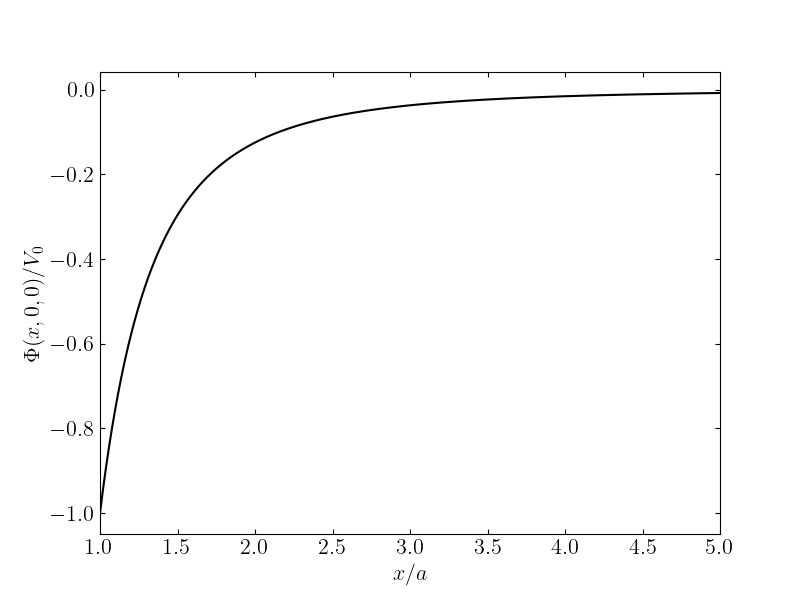
\includegraphics[width=0.7\textwidth]{p2c.png} 
\end{center}

(d) From Coulomb's Law, we can write the full potential as
\begin{equation}
    \Phi=\frac{q}{4\pi\epsilon_0}\qty[\frac1{\abs{\vb{x}-a\zhat}}+\frac1{\abs{\vb{x}+a\zhat}}-\frac2r] 
    =V_0\qty[\frac1{\abs{\vb{x}/a-\zhat}}+\frac1{\abs{\vb{x}/a+\zhat}}-\frac2{r/a}]
\end{equation}
\begin{center}
    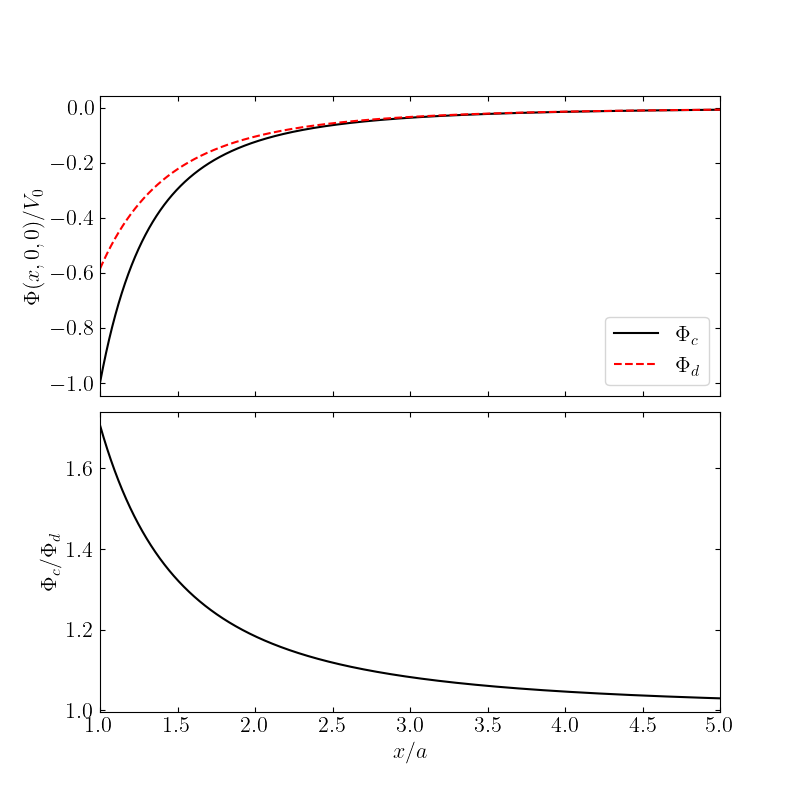
\includegraphics[width=0.7\textwidth]{p2d.png} 
\end{center}
As shown in the above figure, the two potentials agree at $x\gg a$. In the lower
panel, the ratio between them converges to 1 at this limit.
\end{solution}
\end{problem}
%%%%%%%%%%%%%%%%%%%%%%%%%%%%%%%%%%%%%%%%%%%%%%%%%%%%%%%%%%%%%%%%%%%%%%%%%%%%%%%%
%%%%%%%%%%%%%%%%%%%%%%%%%%%%%%%%%%%%%%%%%%%%%%%%%%%%%%%%%%%%%%%%%%%%%%%%%%%%%%%%
\begin{problem}{6.3}[Dipole as derivative of delta function]
A point dipole with dipole moment $\vb{p}$ is located at the point $\vb{x}_0$.
From the properties of the derivative of a Dirac delta function, show that for
calculation of the potential $\Phi$ or the energy of a dipole in an external
field, the dipole can be described by an effective charge density
\begin{equation}\label{p3}
    \rho_{\text{eff}}(\vb{x})=-\vb{p}\vdot\grad\delta(\vb{x}-\vb{x}_0) 
\end{equation}
\begin{solution}
Note that the derivative of the delta function has the following property
\begin{equation}
    \int f(\vb{x}')\grad'\delta(\vb{x}'-\vb{x}_0)d\vb{x}'
    =-\eval{\grad'f(\vb{x}')}_{\vb{x}'=\vb{x}_0}
\end{equation}
Using the density \eqref{p3} to calculate the corresponding potential, we get
\begin{align}
    \Phi(\vb{x})
    &=-\frac{\vb{p}}{4\pi\epsilon_0}\vdot
    \int\frac1{\abs{\vb{x}-\vb{x}'}}\grad'\delta(\vb{x}'-\vb{x}_0)d\vb{x}'\notag\\
    &=\frac1{4\pi\epsilon_0}\vb{p}\vdot
    \eval{\grad'\qty(\frac1{\abs{\vb{x}-\vb{x}'}})}_{\vb{x}'=\vb{x}_0}\notag\\
    &=\frac1{4\pi\epsilon_0}\vb{p}\vdot\frac{\vb{x}-\vb{x}_0}{\abs{\vb{x}-\vb{x}_0}^3}
\end{align}
From (4.10, Jackson), this is the potential due to a dipole moment $\vb{p}$
placed at $\vb{x}_0$.
\end{solution}
\end{problem}
%%%%%%%%%%%%%%%%%%%%%%%%%%%%%%%%%%%%%%%%%%%%%%%%%%%%%%%%%%%%%%%%%%%%%%%%%%%%%%%%
%%%%%%%%%%%%%%%%%%%%%%%%%%%%%%%%%%%%%%%%%%%%%%%%%%%%%%%%%%%%%%%%%%%%%%%%%%%%%%%%
\begin{problem}{6.4}[Nucleus with a quadrupole moment]
A nucleus with quadrupole moment $Q$ finds itself in a cylindrically symmetric
electric field with a gradient $(\partial E_z /\partial z)_0$ along the $z$ axis
at the position of the nucleus.

(a) Show that the energy of quadrupole interaction is
\begin{equation}
    W=-\frac{e}{4}Q\qty(\frac{\partial E_z}{\partial z})_0 
\end{equation}

(b) If it is known that $Q=2\times 10^{-28}$\,\si{m\tothe{2}} and that $W /h$ is
10 \si{MHz}, where $h$ is Planck's constant, calculate $(\partial E_z /\partial
z)_0$ in units of $e /4\pi\epsilon_0a_0^3$, where
$a_0=4\pi\epsilon_0\hbar^2/me^2=0.529\times 10^{-10}$\,\si{m} is the
Bohr radius in hydrogen.

(c) Nuclear charge distributions can be approximated by a constant charge
density throughout a spheroidal volume of semimajor axis $a$ and semiminor axis
$b$. Calculate the quadrupole moment of such a nucleus, assuming that the total
charge is $Ze$. Given that Eu$^{153}$ $(Z=63)$ has a quadrupole moment
$Q=2.5\times 10^{-28}$\,\si{m\tothe{2}} and a mean radius
\begin{equation}
    R=(a+b)/2=7\times10^{-15}\,\si{m} 
\end{equation}
determine the fractional difference in radius $(a-b) /R$.
\begin{solution}
(a) From (4.24, Jackson), the energy is
\begin{align}\label{p4a:W}
    W
    &=-\frac16\qty(
        Q_{11}\eval{\frac{\partial E_x}{\partial x}}_0
        +Q_{22}\eval{\frac{\partial E_y}{\partial y}}_0
        +Q_{33}\eval{\frac{\partial E_z}{\partial z}}_0
    )\notag\\
    &=-\frac{eQ}{6}\qty(
        -\frac12\eval{\frac{\partial E_x}{\partial x}}_0 
        -\frac12\eval{\frac{\partial E_y}{\partial y}}_0 
        +\eval{\frac{\partial E_z}{\partial z}}_0 
    )
\end{align}
where the first and second moment $q$ and $\vb{p}$ are zero because this is a
quadrupole, $Q_{11}=Q_{22}=-(1 /2)Q_{33}$ as written in Jackson, Section 4.2,
and $Q_{33}=eQ$. Now, at the origin, $\eval{\div{\vb{E}}}_0=0$ because there's 
no charge density there. Thus, we can write
\begin{equation}
    -\frac12\qty(\eval{\frac{\partial E_x}{\partial
    x}}_0+\eval{\frac{\partial E_y}{\partial
    y}}_0)=\frac12\eval{\frac{\partial E_z}{\partial z}}_0 
\end{equation}
Plugging this into \eqref{p4a:W} yields
\begin{equation}\label{p4a:W2}
    W=-\frac{eQ}{6}\frac32\eval{\frac{\partial E_z}{\partial z}}_0 
    =-\frac{eQ}{4}\eval{\frac{\partial E_z}{\partial z}}_0
\end{equation}

(b) Inverting \eqref{p4a:W2}, we can write
\begin{align}
    \eval{\frac{\partial E_z}{\partial z}}_0 
    =-\frac{4W}{eQ}
    =-\frac{32\pi^2\epsilon_0\hbar
    (W/h)a_0^3}{e^2Q}\times\frac{e}{4\pi\epsilon_0a_0^3}
    \approx-0.085\qty[\frac{e}{4\pi\epsilon_0a_0^3}]
\end{align}

(c) From the surface of the spheroid, we know that $\abs{z}\leq
a\sqrt{1-r^2 /b^2}=f(r)$. The volume of the spheroid is thus
\begin{equation}
    V=\int_0^b\int_0^{2\pi}\int_{-f(r)}^{f(r)}rdrd\theta dz
    =\frac{4\pi}{3}ab^2
\end{equation}
Thus, the uniform charge density is
\begin{equation}
    \rho=\frac{3Ze}{4\pi ab^2} 
\end{equation}
Then from (4.25, Jackson), we can calculate in cylindrical coordinates
\begin{align}
    Q&=\frac1e\rho\int(2z^2-r^2)rdrd\theta dz\notag\\
     &=\frac{3Z}{ab^2}\int_0^brdr\int_0^{f(r)}(2z^2-r^2)dz\notag\\
     &=\frac{2Z}{5}(a^2-b^2)\notag\\
     &=\frac{252}{5}R(a-b)
\end{align}
Thus,
\begin{equation}
    \frac{a-b}{R}=\frac{5}{252}\frac{Q}{R^2}\approx 0.1 
\end{equation}
\end{solution}
\end{problem}
%%%%%%%%%%%%%%%%%%%%%%%%%%%%%%%%%%%%%%%%%%%%%%%%%%%%%%%%%%%%%%%%%%%%%%%%%%%%%%%%
\end{document}
